%!TEX root = ../main.tex

\RequirePackage{bibentry}
\makeatletter\let\saved@bibitem\@bibitem\makeatother

\documentclass{beamer}
\makeatletter\let\@bibitem\saved@bibitem\makeatother

\renewcommand{\baselinestretch}{1.2}\normalsize
\usetheme{default}
\setbeamertemplate{navigation symbols}{}
\setbeamertemplate{footline}[frame number]

\usepackage{verbatim}
\usepackage{etex}

% BIBLIOGRAPHY APACITE
\usepackage[apaciteclassic]{apacite}
\usepackage{notoccite}
\usepackage{bibentry}
\usepackage{pdfpages}

% MATHEMATICS AND FONTS
\DeclareMathOperator*{\argmin}{arg\,min}
\DeclareMathOperator*{\argmax}{arg\,max}

\renewcommand{\vec}[1]{\mathbf{#1}}

\usepackage{amsfonts}
\usepackage{amsmath}
\usepackage{amssymb}
\usepackage{bbm}
\usepackage{algpseudocode}
\usepackage{setspace}

\usepackage{arev}
\usepackage[latin1]{inputenc}
\usepackage[T1]{fontenc}

\definecolor{darkblue}{rgb}{0,.35,.62}
\definecolor{lightblue}{rgb}{0.8,0.85,1}
\definecolor{lightgrey}{gray}{0.1}	%Farben mischen
\definecolor{Gray}{gray}{0.9}
\definecolor{mplorange}{HTML}{FF7F0E}
\definecolor{mplred}{HTML}{D62728}
\definecolor{mplblue}{HTML}{1F77B4}
\definecolor{mplgreen}{HTML}{2CA02C}

% GRAPHS
\usepackage{graphicx}
\usepackage{subfig}
\usepackage{caption}
\graphicspath{{material/}}
\usepackage{relsize}
\usepackage{lscape}
\usepackage{fancybox}
\usepackage{epstopdf}


% TABLES AND OTHER ENVIRONMENTS
\usepackage{tabularx}
\usepackage{longtable}
\usepackage{booktabs}
\usepackage{color,colortbl}
\usepackage{threeparttable}

\usepackage{enumerate}

\usepackage{fix-cm}

\usepackage{bookmark}
\usepackage{hyperref}
\hypersetup{colorlinks=true,urlcolor=blue,citecolor=black}


\usepackage{tikz}
\tikzset{
	treenode/.style = {shape=rectangle, rounded corners,
		draw, align=center,
		top color=white, bottom color=blue!20},
	root/.style     = {treenode, font=\Large, bottom color=red!30},
	env/.style      = {treenode, font=\ttfamily\normalsize},
	dummy/.style    = {circle,draw}
}
%\usepackage{cmbright}
\def\newblock{\hskip .11em plus .33em minus .07em}
\newcommand{\bs}{\boldsymbol}
\newcommand{\N}{\mathbb{N}}
\newcommand{\cov}{\mathrm{cov}\thin}
\newcommand{\thin}{\thinspace}
\newcommand{\thick}{\thickspace}
\newcommand{\Lim}[1]{\raisebox{0.5ex}{\scalebox{0.8}{$\displaystyle \lim_{#1}\;$}}}

\newcommand{\vect}[1]{\mathbf{#1}}
\newcommand{\myfrac}[3][0pt]{\genfrac{}{}{}{}{\raisebox{#1}{$#2$}}{\raisebox{-#1}{$#3$}}}
\newcommand{\U}{\mathrm{U}}	%Uniform Distribution
\newcommand{\D}{\mathrm{D}}	%Dirichlet Distribution
\newcommand{\W}{\mathrm{W}}	%Wishart Distribution
\newcommand{\E}{\mathrm{E}}		%Expectation
\newcommand{\Prob}{\mbox{Pr}}		%Expectation
\newcommand{\Iden}{\mathbb{I}}	%Identity Matrix
\newcommand{\Ind}{\mathrm{I}}	%Indicator Function
\newcommand{\Tau}{\mathcal{T}\thin}

\newcommand{\var}{\mathrm{var}\thin}
\newcommand{\plim}{\mathrm{plim}\thin}
\newcommand\indep{\protect\mathpalette{\protect\independenT}{\perp}}
\def\independenT#1#2{\mathrel{\rlap{$#1#2$}\mkern5mu{#1#2}}}
\newcommand{\notindep}{\ensuremath{\perp\!\!\!\!\!\!\diagup\!\!\!\!\!\!\perp}}%

\newcommand{\mc}{\multicolumn}

\newcommand{\ph}{\phantom}
% weitere Optionen:
% secbar: Gliederung im Kopf, nur sections (alternativ zu subsecbar)
% handout: Produktion von Handouts, keine Animationen
\definecolor{darkblue}{rgb}{0,.35,.62}
\definecolor{lightblue}{rgb}{0.8,0.85,1}
\definecolor{lightgrey}{gray}{0.1}	%Farben mischen

%	kbordermatrix options

\makeatletter
\newcommand{\vast}{\bBigg@{4}}
\newcommand{\Vast}{\bBigg@{5}}
\makeatother
\newcommand{\indicator}[1]{\mathbbm{1}{\left\{ {#1} \right\} }}
\newcommand{\indic}{1{\hskip -2.5 pt}\hbox{1} }


\definecolor{lightgrey}{gray}{0.90}	%Farben mischen
\definecolor{grey}{gray}{0.85}
\definecolor{darkgrey}{gray}{0.65}
\definecolor{lightblue}{rgb}{0.8,0.85,1}

\renewcommand{\arraystretch}{1.5}


\usepackage{tikz}
\usetikzlibrary{trees,shapes,arrows,decorations.pathmorphing,backgrounds,positioning,fit,petri}
\renewcommand*{\familydefault}{\sfdefault}

\tikzset{forestyle/.style = {rectangle, thick, minimum width = 5cm, minimum height = 0.5cm, text width = 4.5cm, outer sep = 1mm},
	pre/.style={<-, shorten <=1pt, >=stealth, ultra thick},
	extend/.style={<-,dashed, shorten <=1pt, >=stealth, ultra thick}}
\captionsetup[subfigure]{labelformat=empty}


\newcommand{\beginbackup}{
	\newcounter{framenumbervorappendix}
	\setcounter{framenumbervorappendix}{\value{framenumber}}
}
\newcommand{\backupend}{
	\addtocounter{framenumbervorappendix}{-\value{framenumber}}
	\addtocounter{framenumber}{\value{framenumbervorappendix}}
}


% Begin Full Justification ---------------------------------------------------------

\usepackage{ragged2e}
% \usepackage{etoolbox}
\usepackage{lipsum}
\makeatletter
\renewcommand{\itemize}[1][]{%
	\beamer@ifempty{#1}{}{\def\beamer@defaultospec{#1}}%
	\ifnum \@itemdepth >2\relax\@toodeep\else
	\advance\@itemdepth\@ne
	\beamer@computepref\@itemdepth% sets \beameritemnestingprefix
	\usebeamerfont{itemize/enumerate \beameritemnestingprefix body}%
	\usebeamercolor[fg]{itemize/enumerate \beameritemnestingprefix body}%
	\usebeamertemplate{itemize/enumerate \beameritemnestingprefix body begin}%
	\list
	{\usebeamertemplate{itemize \beameritemnestingprefix item}}
	{\def\makelabel##1{%
			{%
				\hss\llap{{%
						\usebeamerfont*{itemize \beameritemnestingprefix item}%
						\usebeamercolor[fg]{itemize \beameritemnestingprefix item}##1}}%
			}%
		}%
	}
	\fi%
	\beamer@cramped%
	\justifying% NEW
	%\raggedright% ORIGINAL
	\beamer@firstlineitemizeunskip%
}

\justifying

% \apptocmd{\frame}{\justifying}{}{}

\usepackage{array}
\newcolumntype{L}[1]{>{\raggedright\let\newline\\\arraybackslash\hspace{0pt}}m{#1}}
\newcolumntype{C}[1]{>{\centering\let\newline\\\arraybackslash\hspace{0pt}}m{#1}}
\newcolumntype{R}[1]{>{\raggedleft\let\newline\\\arraybackslash\hspace{0pt}}m{#1}}



% End Full Justification ------------------------------------------------------------


%!TEX root = ../main.tex
\title{Returns to Education}
\author{Philipp Eisenhauer}

\date{}

\let\otp\titlepage
%\renewcommand{\titlepage}{\otp\addtocounter{framenumber}{-1}}

\begin{document}
\maketitle

 \begin{frame}

 I heavily draw on the material presented in:

\begin{itemize}
\item \bibentry{Heckman.2006a}
\end{itemize}

\end{frame}


 \begin{frame}
We will look at two papers that explore reduced-form estimations of the returns to education
.
\begin{itemize}
\item \bibentry{Carneiro.2002}
\item \bibentry{Mogstad.2017}
\end{itemize}
 \end{frame}

 \begin{frame}
We will look at two papers that explore structural estimations of the returns to education
.
\begin{itemize}
\item \bibentry{Cunha.2005b}
\item \bibentry{Eisenhauer.2015b}
\end{itemize}
 \end{frame}


\begin{frame}
Why are returns to education important?
\begin{itemize}
\item help explain wage inequality
\item judge relative profitability of investment in education?
\item ...
\end{itemize}
\end{frame}

\begin{frame}\nocite{Mincer.1958,Mincer.1974}
\textbf{Mincer Equation}
\begin{align*}
Y(s, x) = \alpha + \rho_s s + \beta_0 x + \beta_1 x^2 + \epsilon
\end{align*}

Conceptual Frameworks
\begin{itemize}
\item compensating differences model
\item accounting-identity model
\end{itemize}
\end{frame}

%-------------------------------------------------------------------------------
%-------------------------------------------------------------------------------
\begin{frame}\begin{center}
\LARGE\textit{Compensating Differences Model}
\end{center}\end{frame}

\begin{frame}
\begin{align*}
V(s) = Y(s)\int_s^T e^{-rt} dt = \frac{Y(s)}{r}(e^{-rs} - e^{-rT})
\end{align*}

\end{frame}

\begin{frame}

Equalizing present value of earnings across schooling levels:
\begin{align*}
\ln Y(s) = \ln Y(0) + r s + \ln\left(\frac{1 -e^{-rs}}{1 - e^{-r(T - s)}}\right) \\
\end{align*}

$\Rightarrow$ $\rho_s$ equals the market interest rate

\end{frame}

\begin{frame}
Model Features:
\begin{itemize}
\item identical abilities and opportunities
\item no credit constraints
\item perfect certainty
\item no direct cost of schooling
\item no nonpecuniary benefits of school and work
\end{itemize}
\end{frame}


\begin{frame}
Model Features:
\begin{itemize}
\item identical abilities and opportunities
\item no credit constraints
\item perfect certainty
\item no direct cost of schooling
\item no nonpecuniary benefits of school and work
\end{itemize}
\end{frame}

%-------------------------------------------------------------------------------
%-------------------------------------------------------------------------------
\begin{frame}\begin{center}
\LARGE\textit{Accounting-Identity Model}
\end{center}\end{frame}

\begin{frame}
\begin{align*}
P_t & \equiv P_{t - 1} (1 + k_{t - 1} \rho_{t - 1}) \equiv \prod^{t - 1}_{j= 0} (1 + \rho_jk_j)P_0 \\
& \\
\ln P_t & \equiv \ln P_0  + s \ln(1 + \rho_s) + \sum^{t -1}_{j=2} \ln(1 + \rho_0 k_j) \\
& \approx  \ln P_0 + s \rho_s + \rho_0 \sum^{t - 1}_{j=s} k_j
\end{align*}
\end{frame}



\begin{frame}
Assuming linearly declining rate of post-school investment:
\begin{align*}
k_{s + x} = \kappa\left( 1 - \frac{x}{T}\right),\text{where} \quad x = t - s
\end{align*}
\end{frame}

\begin{frame}
\begin{figure}[htp]\centering
\caption{Post-School Investment}\label{Post-School Investment}\scalebox{0.50}{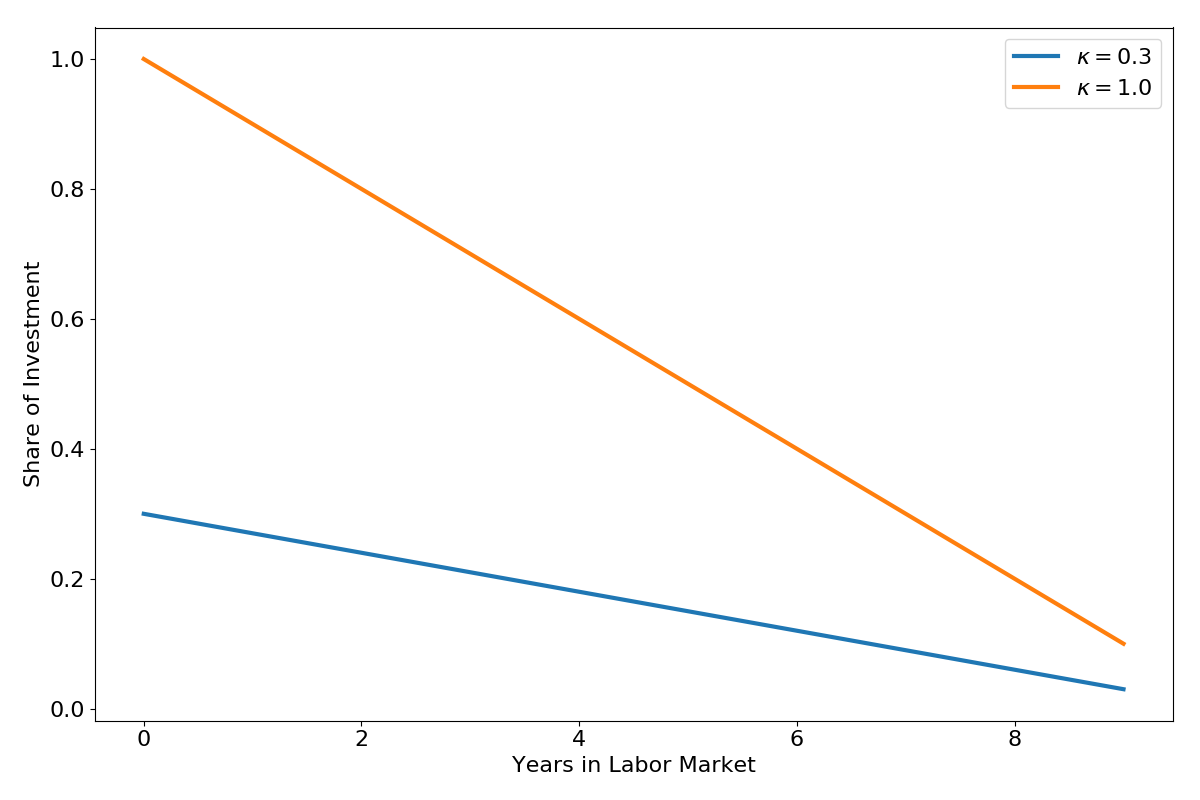
\includegraphics{fig-mincer-post-school}}
\end{figure}
\end{frame}

\begin{frame}
\begin{align*}
\ln P_{x + s} \approx \ln P_0 + s\rho_s + \left(\rho_0 \kappa + \frac{\rho_0\kappa}{2T}\right)x - \frac{\rho_0\kappa}{2T} x^2 \\
\end{align*}
Accounting for the difference in potential and observed earnings:
\begin{align*}
\ln Y(s, x) & = \ln P_{x + s} - \kappa\left(1 - \frac{x}{T}\right) \\
            & = [\ln P_0 - \kappa] + \rho_s s + \left(\rho_0\kappa + \frac{\rho_0\kappa}{2T} + \frac{\kappa}{T}\right) x - \frac{\rho_0\kappa}{2T}x^2
\end{align*}
$\Rightarrow$ $\rho_s$ is the average earnings increase with schooling
\end{frame}

\begin{frame}
\textbf{Standard Mincer Equation}
\begin{align*}
\ln Y(s, x) = \alpha + \rho_s s + \beta_0 x + \beta_1 x^2,
\end{align*}
where
\begin{align*}
\alpha & =\ln P_0 - \kappa \\
\beta_0 & = \left(\rho_0\kappa + \frac{\rho_0\kappa}{2T} + \frac{\kappa}{T}\right) \\
\beta_1 & = \frac{\rho_0\kappa}{2T}
\end{align*}
\end{frame}

\begin{frame}
\textbf{Random Coefficient Version}
\begin{align*}
\ln Y(s_i, x_i) = \alpha_{i} + \rho_{si} s_i + \beta_{0i} x_i + \beta_{1i} x_i^2
\end{align*}
and let
\begin{align*}
\bar{\alpha} = \E[\alpha_i] &\qquad \bar{\rho}_s = \E[\rho_{si}]\\
\bar{\beta}_0 = \E[\beta_{0i}]&\qquad \bar{\beta}_1 = \E[\beta_{1i}]
\end{align*}
\end{frame}


\begin{frame}
Dropping individual subscripts ...
\begin{align*}
\ln Y(s, x) & = \bar{\alpha} + \bar{\rho}_s s + \bar{\beta}_{0} x + \bar{\beta}_{1} x^2 \\
                & + \underbrace{[(\alpha - \bar{\alpha}) + (\rho_s - \bar{\rho}_s) s + (\beta_0 - \bar{\beta}_0)x + (\beta_1 - \bar{\beta}_1)x^2 ]}_{\epsilon}\\
\end{align*}
$\Rightarrow$ If the schooling decision is determined by individual returns, then we are back in the case of a correlated random coefficient model \citep{Heckman.2006d}.
\end{frame}



\begin{frame}[plain]

\begin{center}
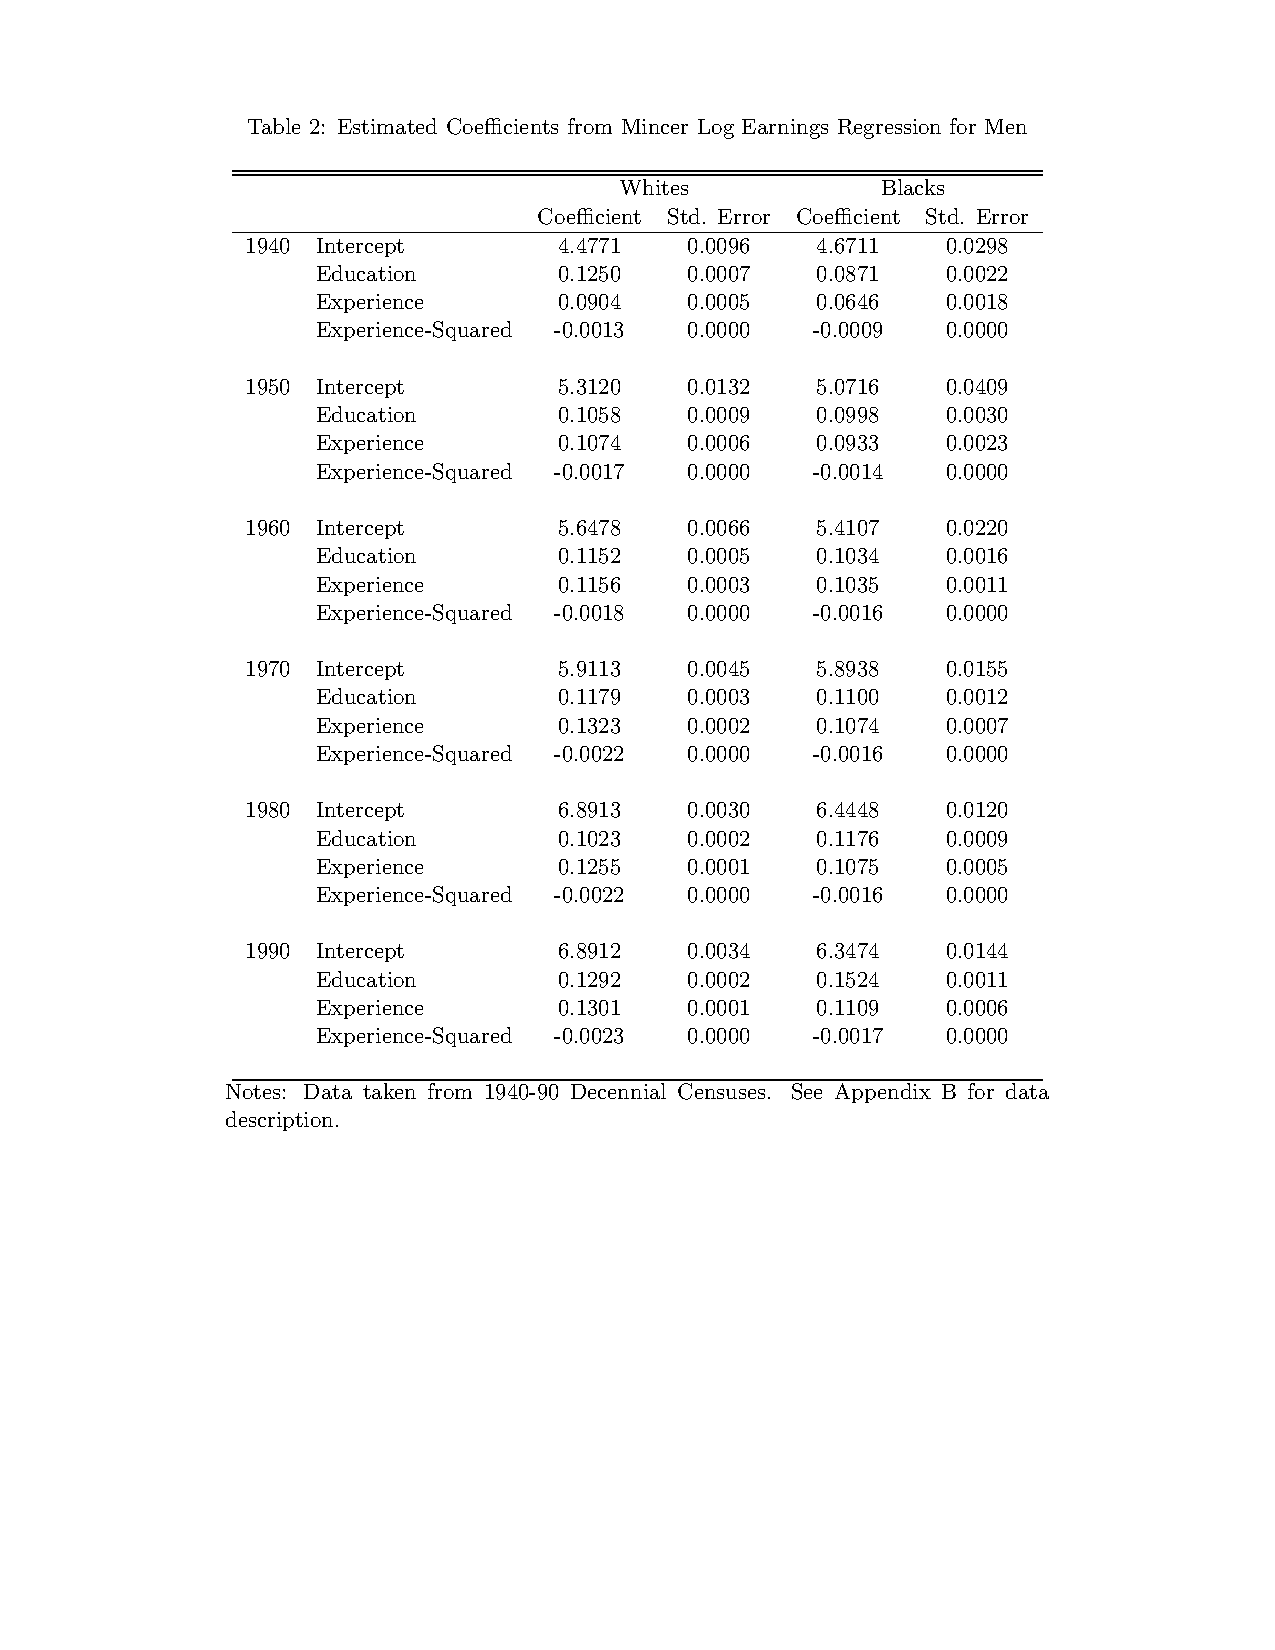
\includegraphics[width=.65\columnwidth]{fig-mincer-regressions}
\end{center}

\end{frame}

%-------------------------------------------------------------------------------
%-------------------------------------------------------------------------------
\begin{frame}\begin{center}
\LARGE\textit{Implications}
\end{center}\end{frame}



\begin{frame}
\begin{itemize}
\item Log-earnings profiles are parallel across schooling levels.
\begin{align*}
\frac{\partial \ln Y(s, x)}{\partial s \partial x} = 0
\end{align*}
\item Log-earnings age profiles diverge with age across schooling levels.
\begin{align*}
\frac{\partial \ln Y(s, x)}{\partial s \partial t} = \frac{\rho_0\kappa}{T} > 0
\end{align*}
\item The variance of earnings over the life cycle has a U-shaped pattern.
\end{itemize}
\end{frame}


\begin{frame}
\begin{figure}[htp]\centering
\caption{Mincerian Experience Profiles}\label{Mincerian Experience Profiles}\scalebox{0.3}{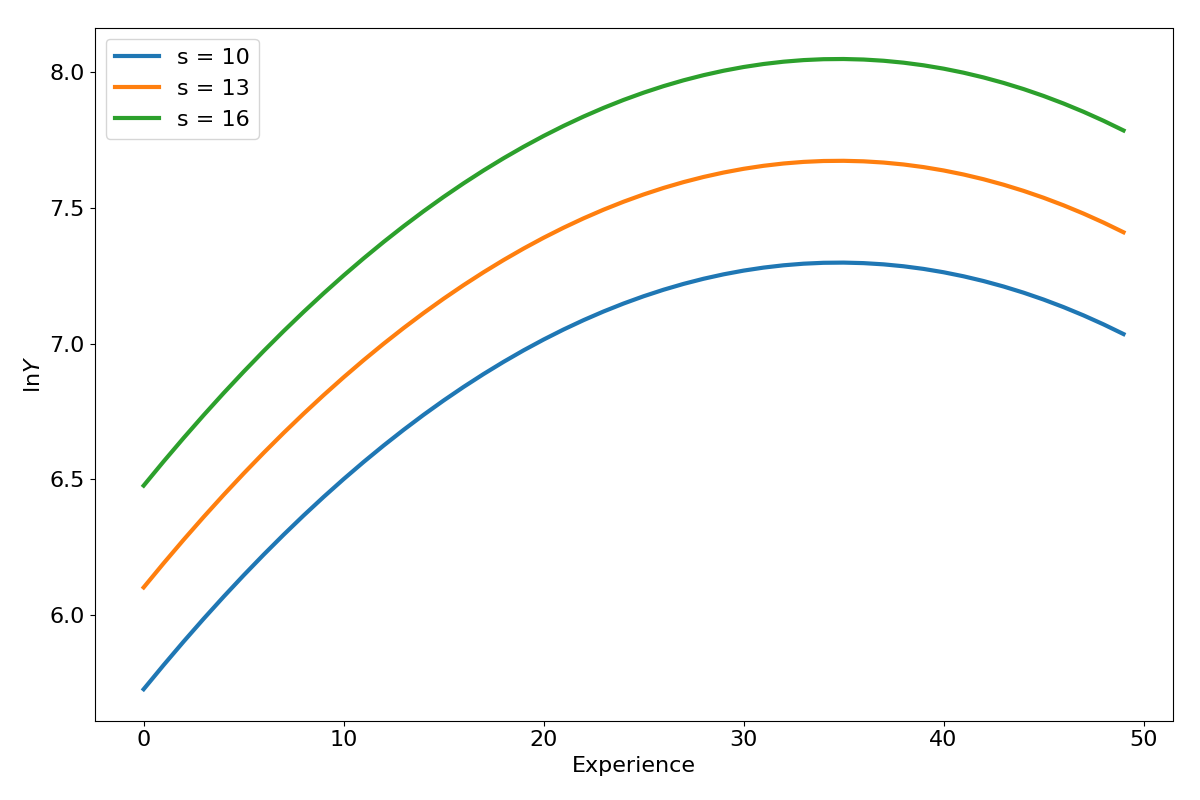
\includegraphics{fig-mincer-equation-experience}}
\end{figure}
\end{frame}

\begin{frame}
\begin{figure}[htp]\centering
\caption{Mincerian Age Profiles}\label{Mincerian Age Profiles}\scalebox{0.3}{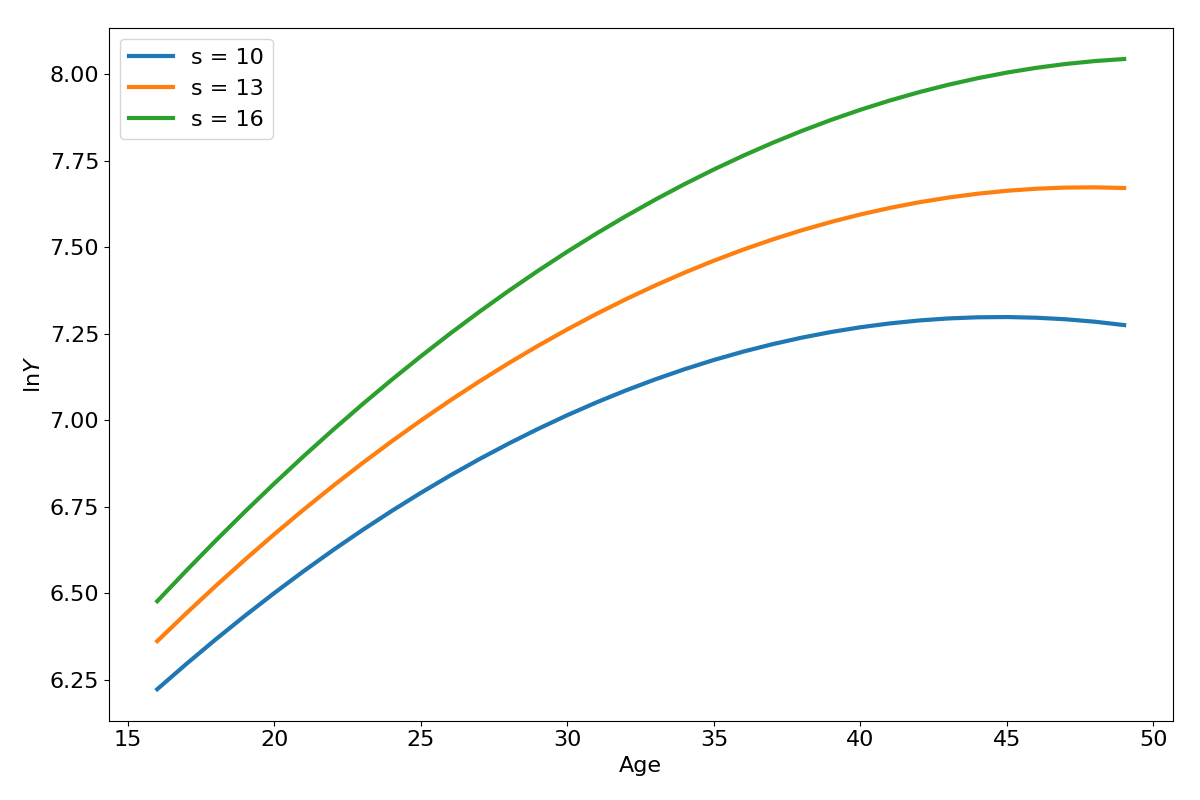
\includegraphics{fig-mincer-equation-age}}
\end{figure}
\end{frame}


%-------------------------------------------------------------------------------
%-------------------------------------------------------------------------------
\begin{frame}\begin{center}
\LARGE\textit{Empirical Evidence}
\end{center}\end{frame}

\begin{frame}[plain]
\begin{center}
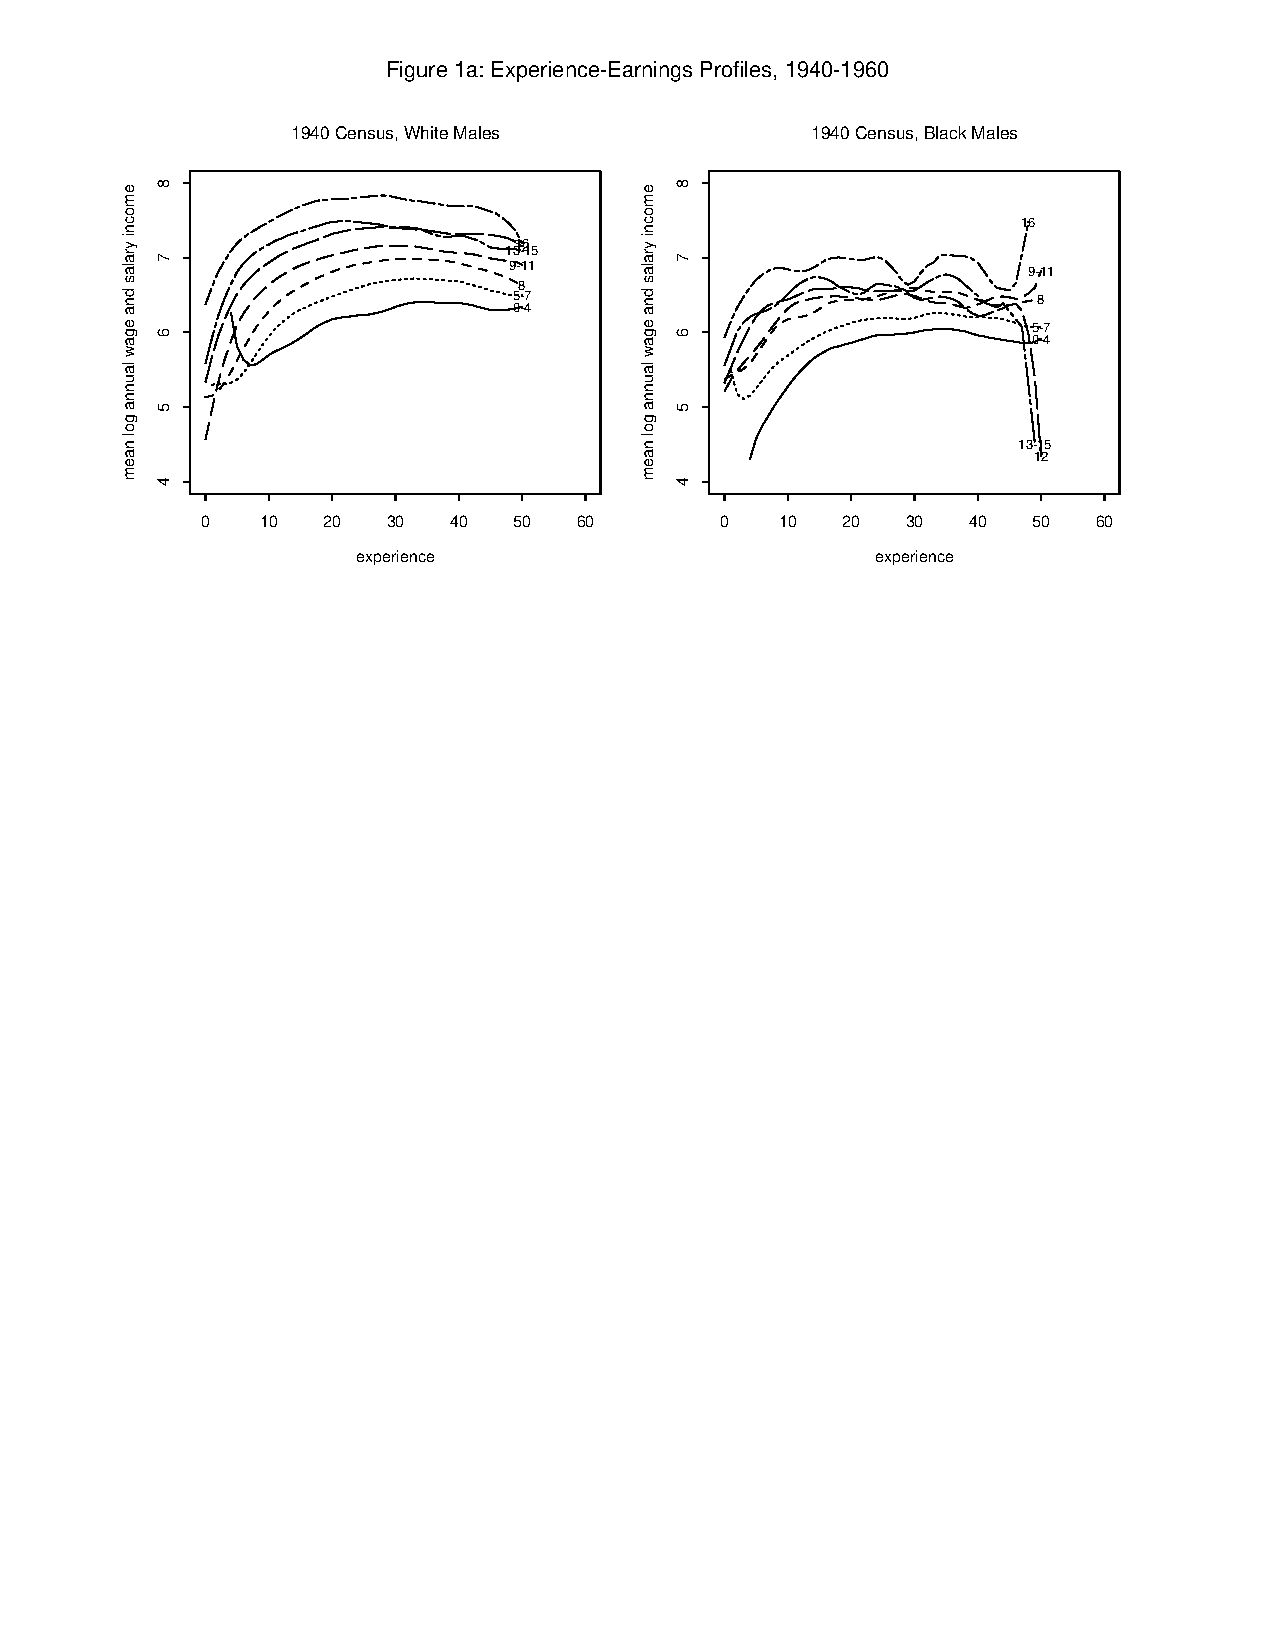
\includegraphics[width=.90\columnwidth]{fig-mincer-experience-1940}
\end{center}
\end{frame}

\begin{frame}[plain]
\begin{center}
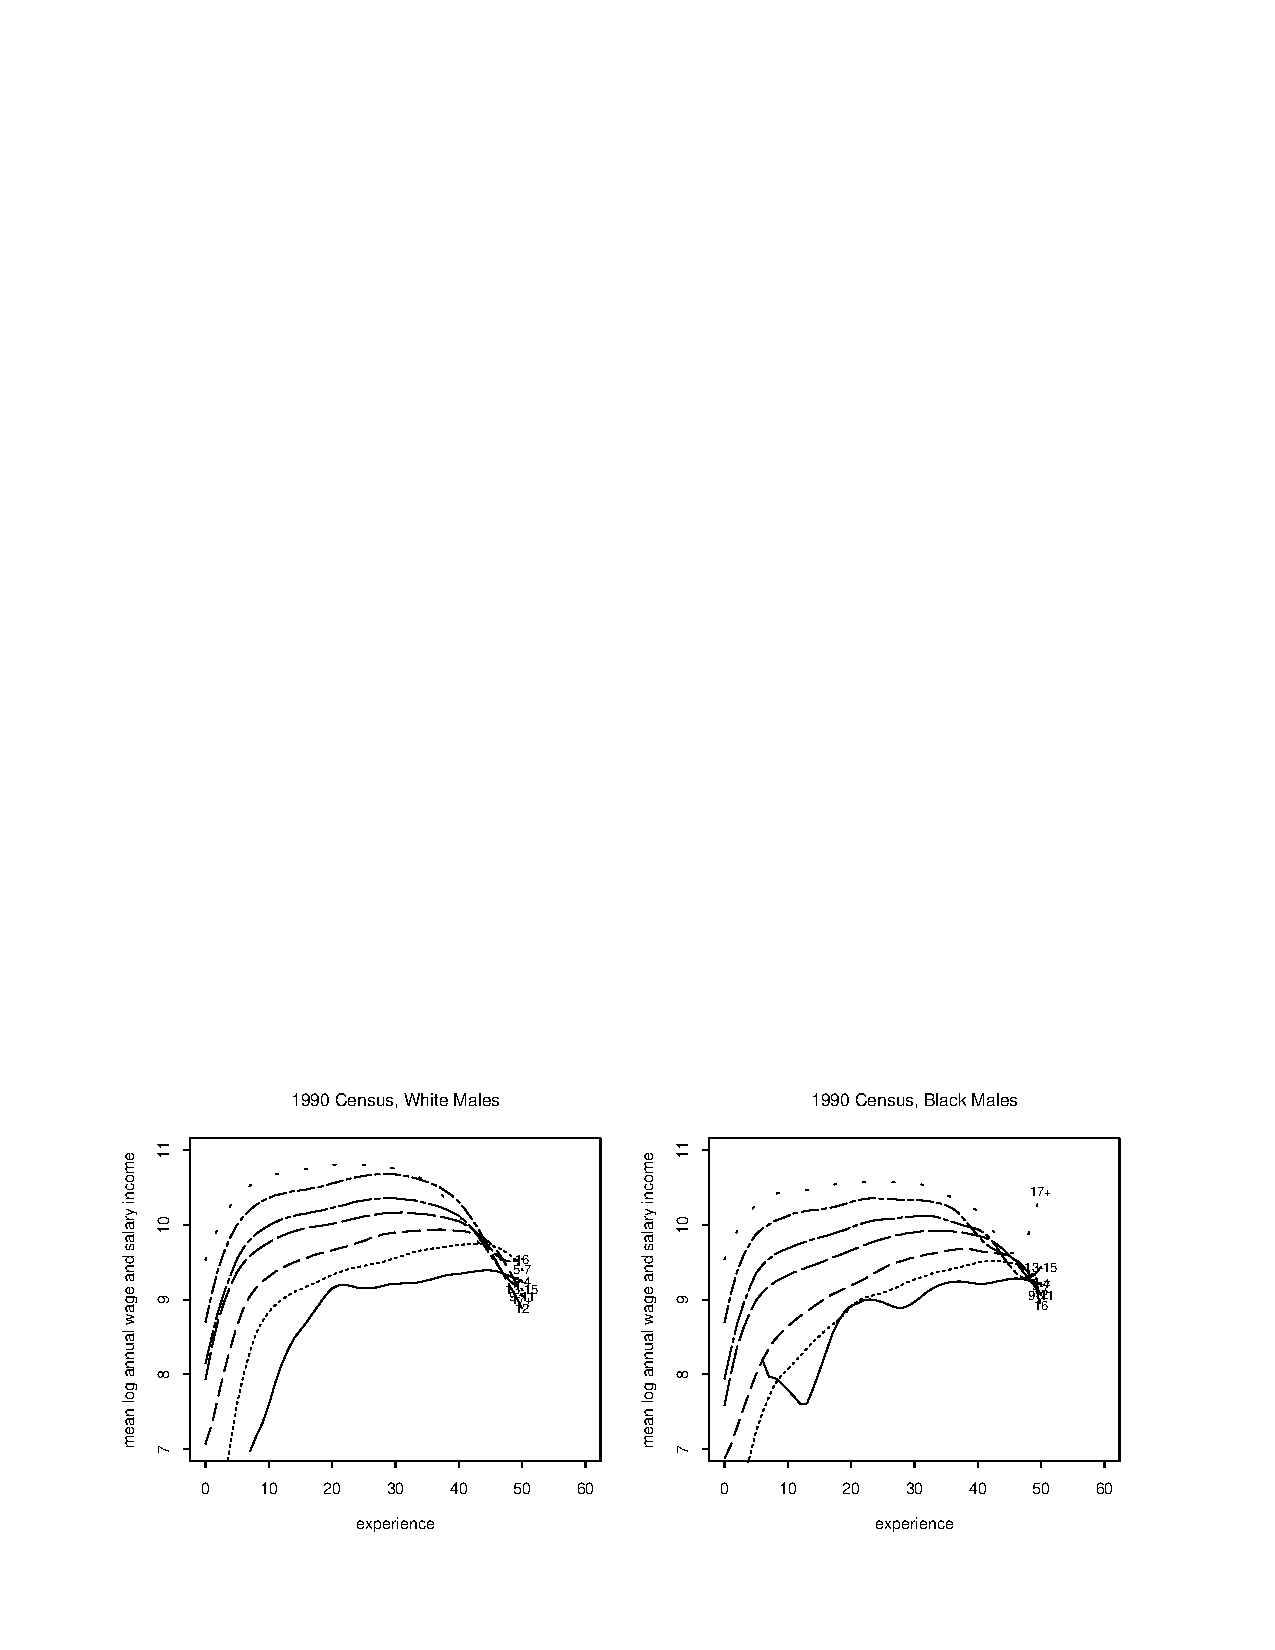
\includegraphics[width=.90\columnwidth]{fig-mincer-experience-1990}
\end{center}
\end{frame}

\begin{frame}[plain]
\begin{center}
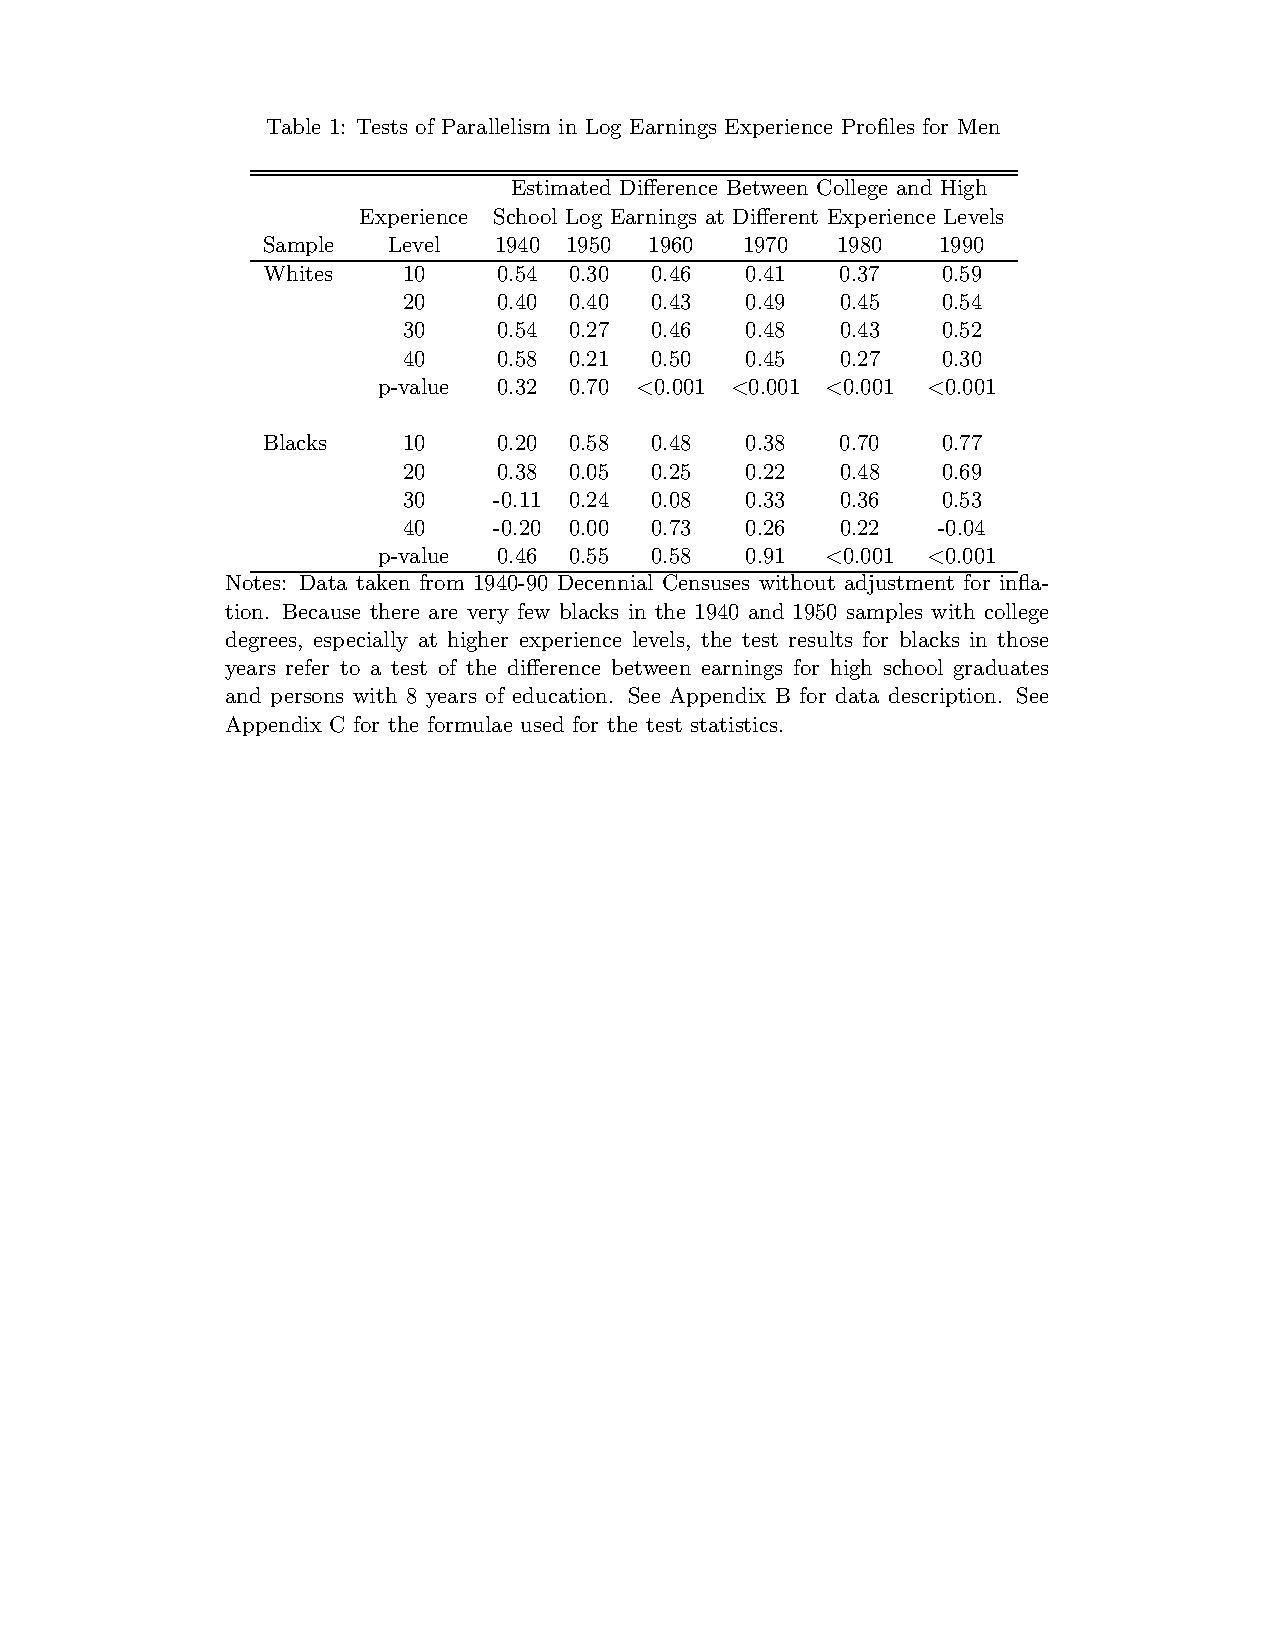
\includegraphics[width=.90\columnwidth]{fig-mincer-parallelism}
\end{center}
\end{frame}

\begin{frame}[plain]
\begin{center}
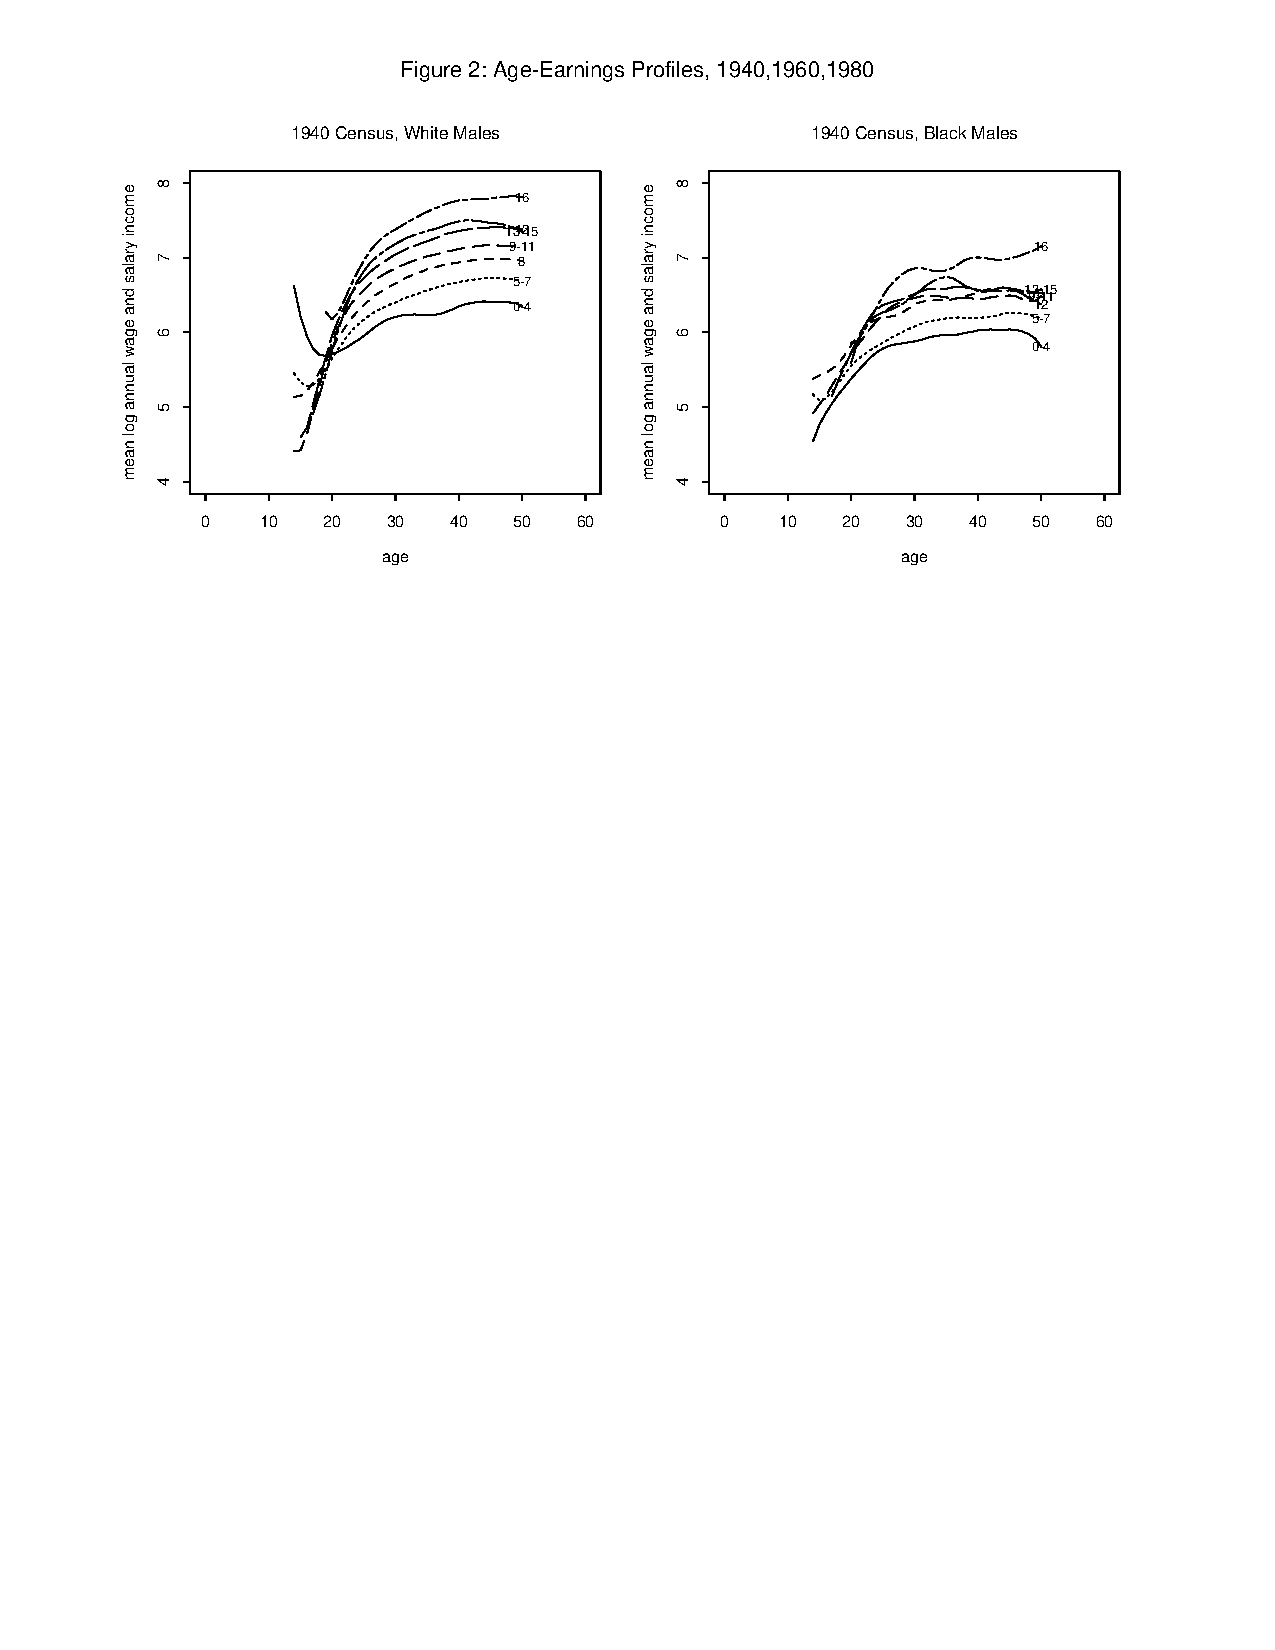
\includegraphics[width=.90\columnwidth]{fig-mincer-age-1940}
\end{center}
\end{frame}

\begin{frame}[plain]
\begin{center}
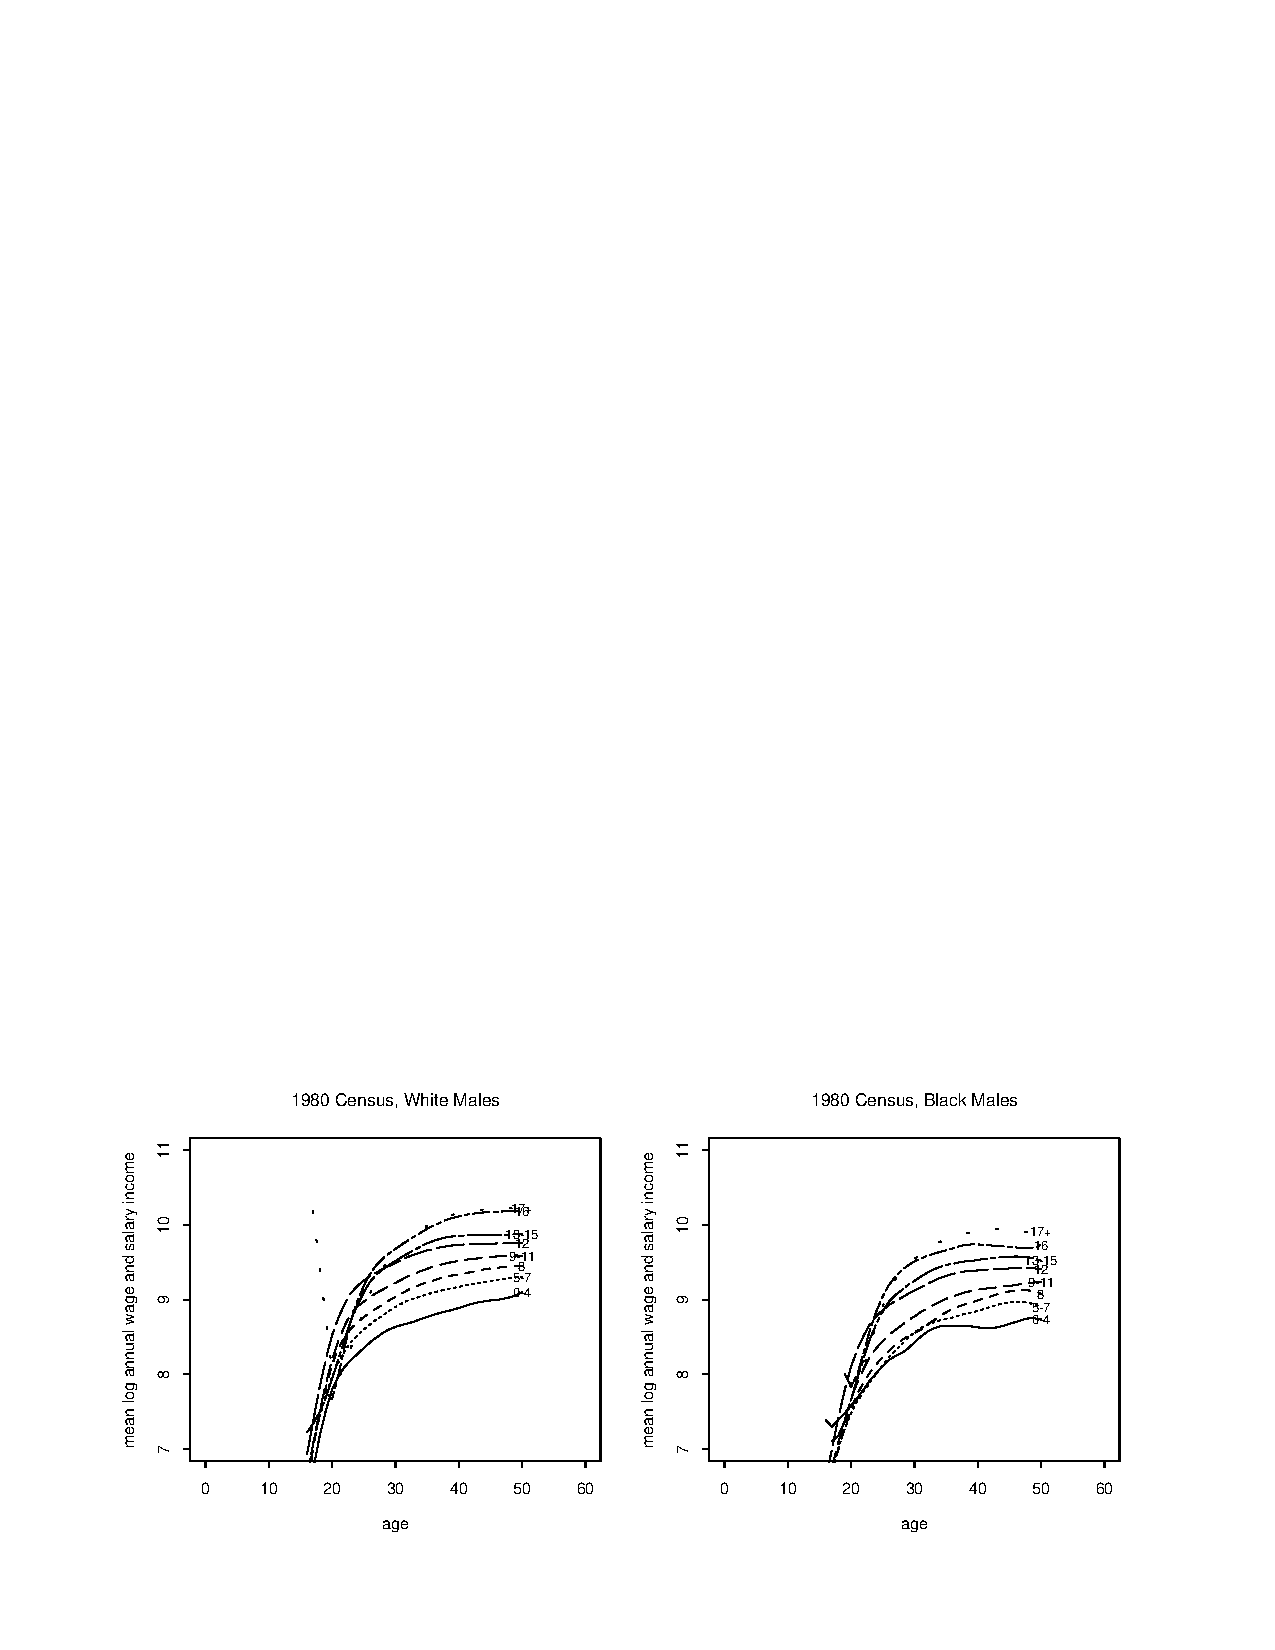
\includegraphics[width=.90\columnwidth]{fig-mincer-age-1980}
\end{center}
\end{frame}

\begin{frame}[plain]
\begin{center}
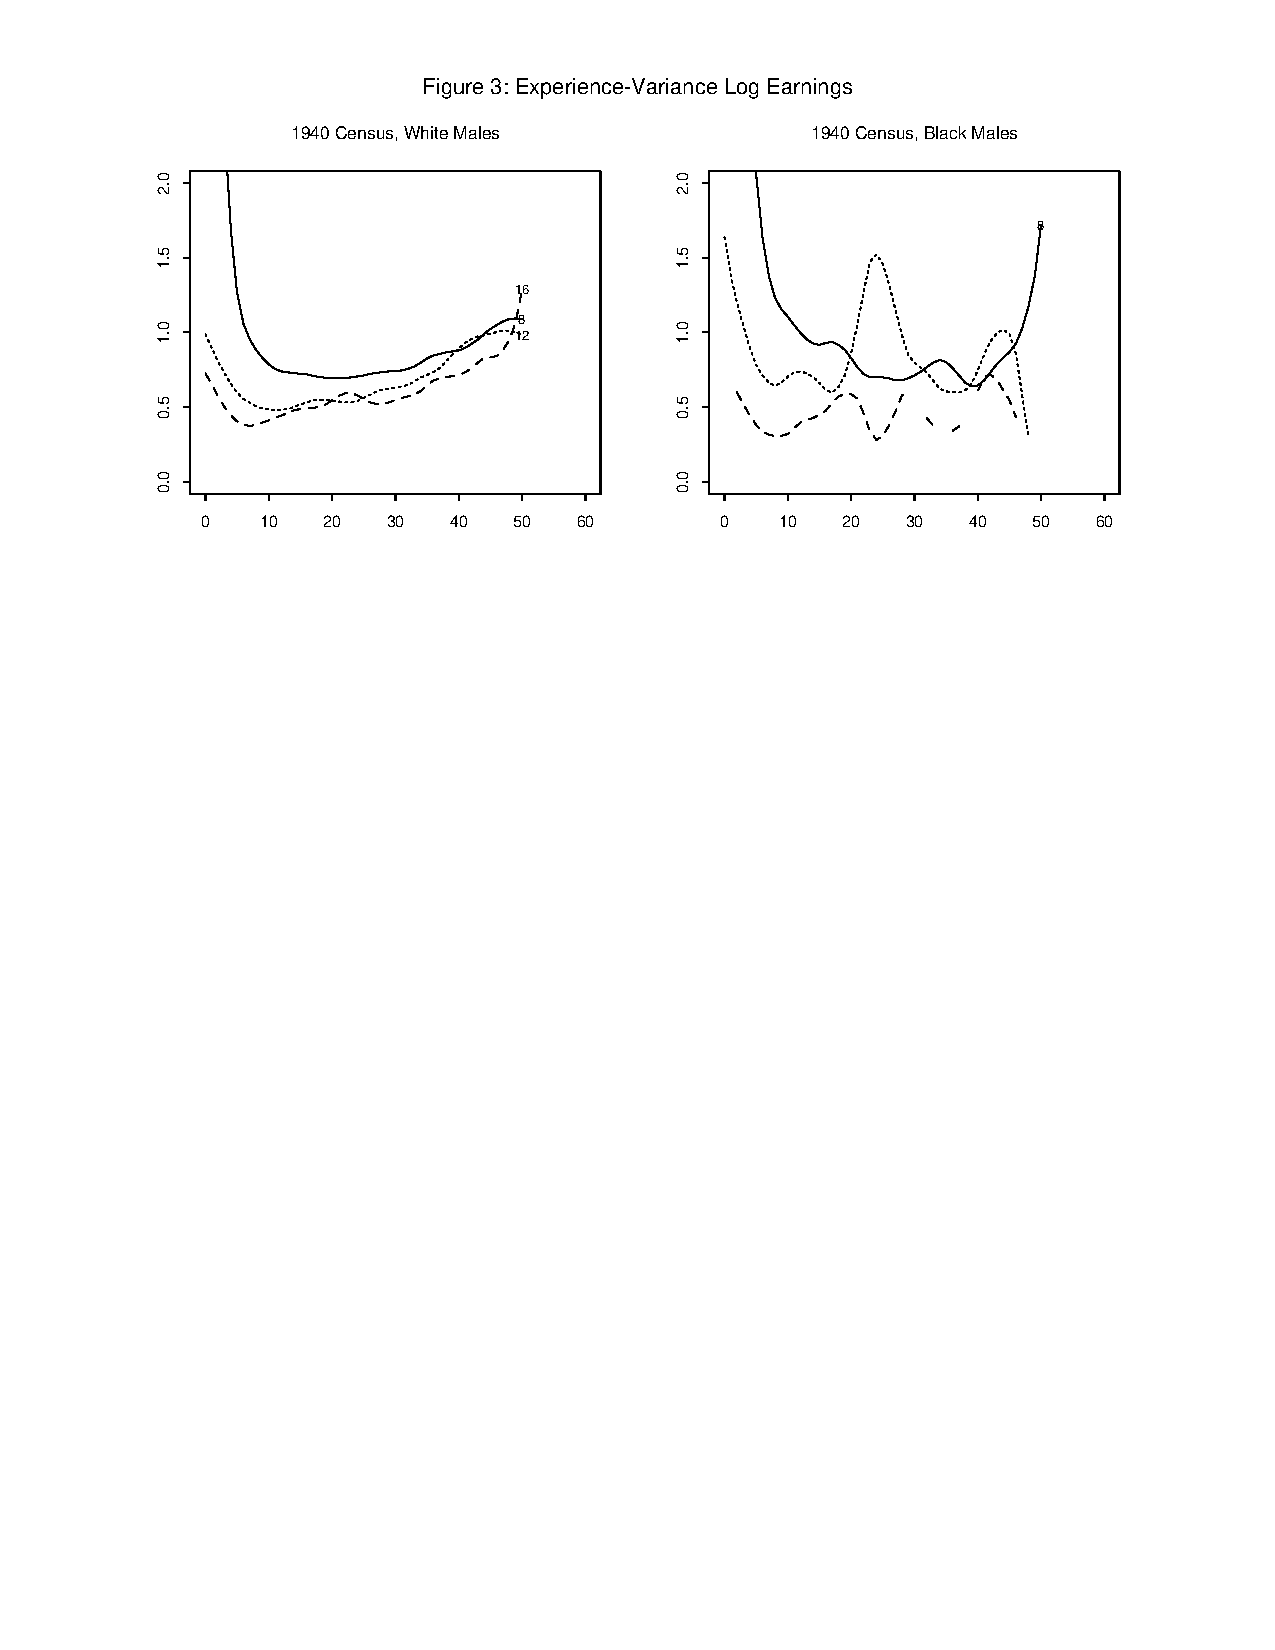
\includegraphics[width=.90\columnwidth]{fig-mincer-variance-1940}
\end{center}
\end{frame}

\begin{frame}[plain]
\begin{center}
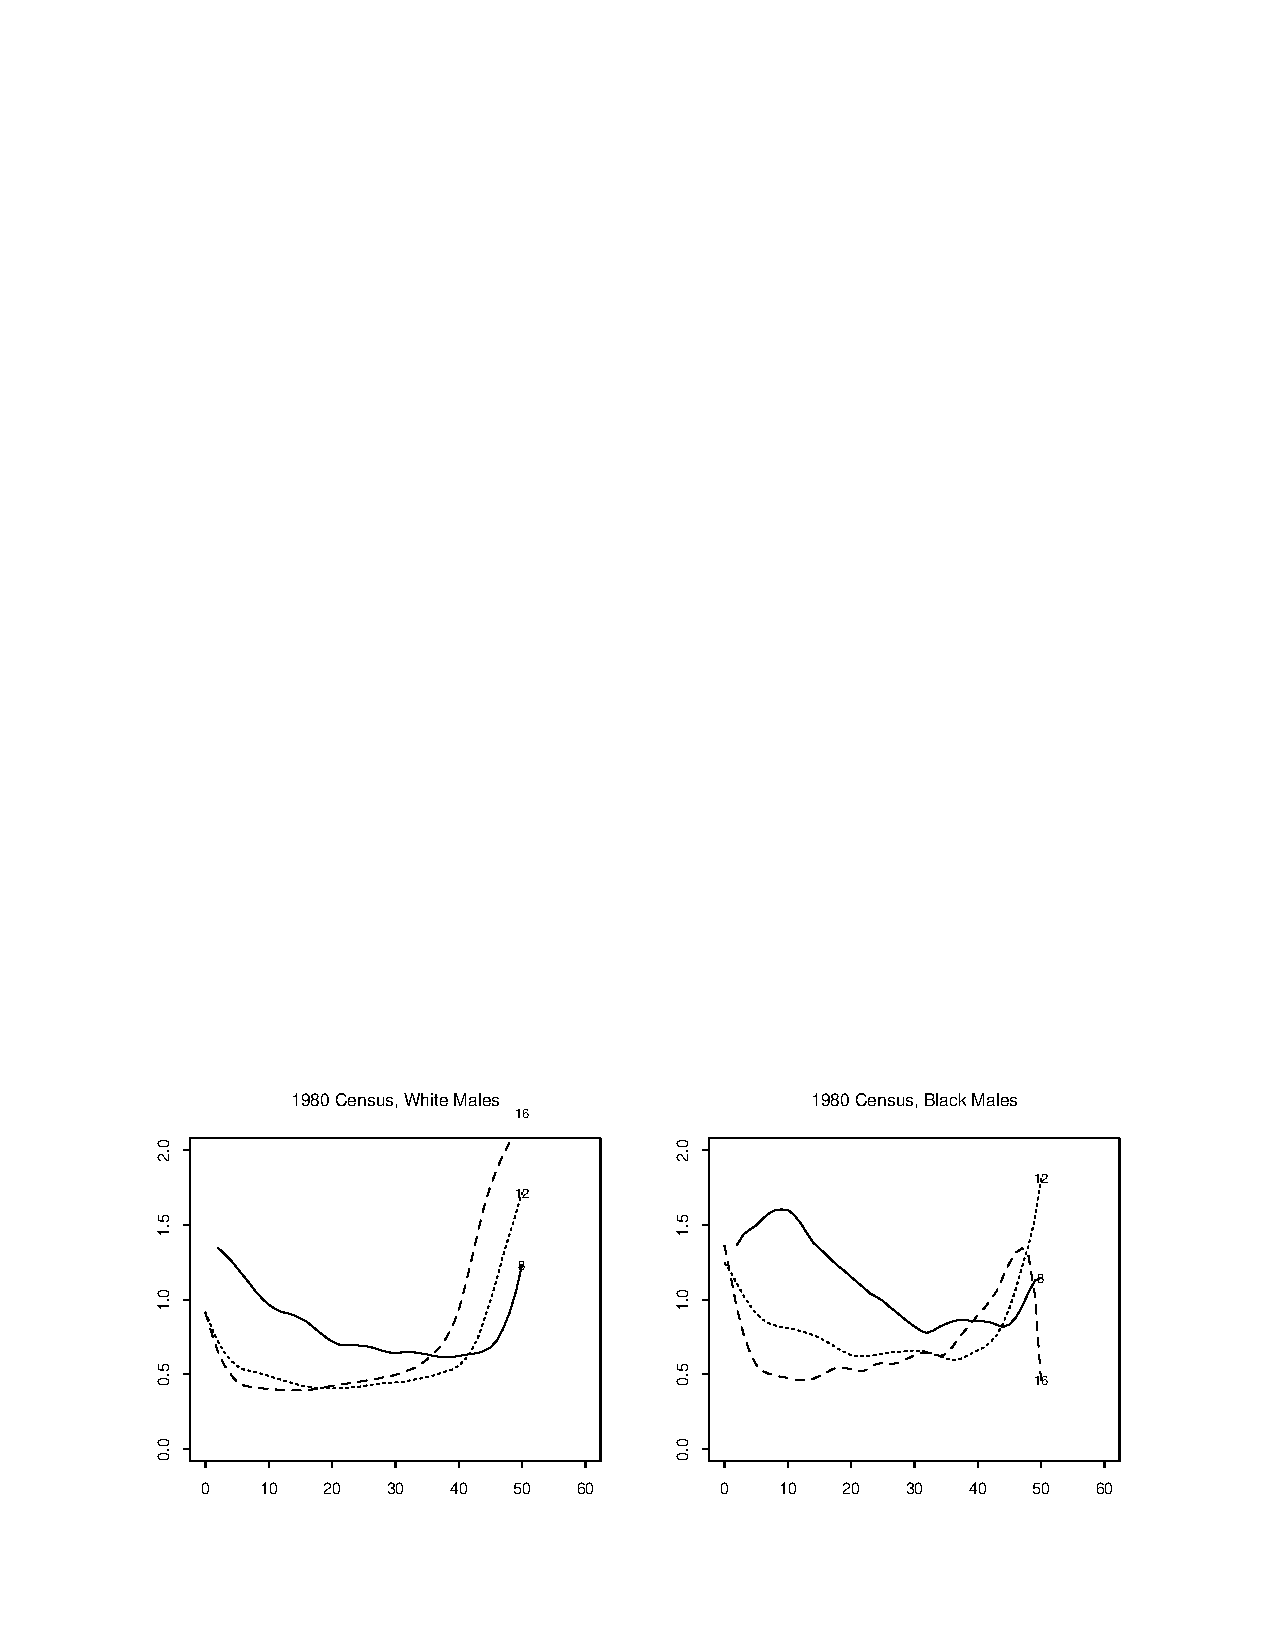
\includegraphics[width=.90\columnwidth]{fig-mincer-variance-1980}
\end{center}
\end{frame}

%!TEX root = ../main.tex
\beginbackup\appendix
\begin{frame}\begin{center}
\LARGE\textbf{Appendix}
\end{center}\end{frame}

%------------------------------------------------------------------------------
%------------------------------------------------------------------------------
\begin{frame}\begin{center}
\LARGE\textit{References}
\end{center}\end{frame}
%------------------------------------------------------------------------------
%------------------------------------------------------------------------------
\newgeometry{margin=1cm}
\begin{frame}[allowframebreaks]\frametitle{}

\nocite{Carneiro.2011}

\bibliographystyle{apalike}
\bibliography{../../submodules/bibliography/literature}


\end{frame}

\backupend
\end{document}
